\documentclass[12pt,a4paper]{article}
\linespread{1.1}
\usepackage[utf8x]{inputenc}
\usepackage{ucs}
\usepackage{amsmath}
\usepackage{bm}
\usepackage{amsfonts}
\usepackage{amssymb}
\usepackage{graphicx}
\usepackage{wrapfig}
\usepackage{lipsum}
\usepackage[hidelinks]{hyperref}
\usepackage{indentfirst}
\usepackage[margin=1cm]{caption}
\usepackage{siunitx}

\usepackage[superscript, nomove]{cite}

\makeatletter
\renewcommand{\@citess}[1]{\textsuperscript{[#1]}}
\makeatother

\newcommand{\citein}[1]{[\citen{#1}]}

\usepackage[left=2.2cm, right=2.2cm, top=2.2cm, bottom=2.2cm]{geometry}

\usepackage[svgnames]{xcolor}
\definecolor{blue}{RGB}{13,71,161}

\usepackage{chemformula}

\author{Jakub Bartosz Dranczewski}
\title{Designing, Simulating, and Optimising Nanoantennas that utilise Nonlinear Effects}
\date{}
\begin{document}

\begin{titlepage}
	\vspace*{-0.65in}
	\hspace*{-.72in}
	
\includegraphics[width=0.5\textwidth]{img/Imperial-logo.pdf}
	\begin{center}
		\vspace*{2cm}
		
		\Huge
		\textbf{Designing, Simulating, and Optimising Nanoantennas that utilise Nonlinear Effects}
		
		\Large
		A literature review
		
		\vspace{1.2cm}
		\large
		Project: EXSS-Sapienza-1\\
		Project partner: Taran Attavar\\
		Supervisor: Riccardo Sapienza\\
		Assessor: Cynthia Vidal
		
		\vspace{1.5cm}
		
		\textbf{Jakub Bartosz Dranczewski}
		
		\vfill
		
		\vspace{0.4cm}
		
		
		Word count: 2400 %TODO update this of course!
		
	\end{center}
\end{titlepage}

\begin{abstract}
Nonlinear optics is a field of research concerned with the effects that arise when electric fields in materials are large enough that the polarisation is no longer directly proportional to the electric field. Nanoantennas are an emerging method of bringing these effects to a smaller scale, with hopes that this allows for eventual easier integration in optical devices. This review presents an introduction to the above concepts, a number of examples of research into optimising the output of nonlinear generation, and a method of computationally predicting this output in order to inform experimental investigation.
\end{abstract}

\section{Introduction}
The goal of our project is to investigate, both experimentally and computationally, the applicability and efficiency of different nanoantenna designs for enhancing nonlinear optical effects at the nanoscale. Light manipulation using the nonlinear response of materials has existing and promising future applications in a number of areas, including frequency control for laser light, optical communications, spectroscopy, data storage, and sensing\cite{garmireNonlinearOpticsDaily2013a}. Nonlinear effects often require large interaction volumes and high laser powers to occur, and nanoantennas are one of the proposed ways to alleviate this and bring nonlinear optics to small-scale applications.

\section{Nonlinear optics}
\label{section:nonlinear-optics}
When considering the propagation of light in matter, it is often assumed that the response of the material is linear\cite{jacksonClassicalElectrodynamics1999}, giving a simple expression for the polarisation:
\begin{equation}
	\label{eq:linear-polarisation}
	\bm{P}=\epsilon_0\chi\bm{E},
\end{equation}
with $\epsilon_0$ being the permittivity of free space, $\chi$ the linear electric susceptibility, and $\bm{E}$ the electric field. As outlined in \citein{boydNonlinearOptics2008}, this expression can be generalised to include terms that only gain significance at higher field magnitudes, and can be understood as the atomic potentials for the electrons in the material deviating from the simple harmonic approximation:
\begin{equation}
\begin{aligned}
	\label{eq:nonlinear-polarisation}
	P_i&=\epsilon_0(\chi^{(1)}E_i+\chi^{(2)}E_i^2+\chi^{(3)}E_i^3+...)\\
	&=P_i^{(1)}+P_i^{(2)}+P_i^{(3)}+...,
\end{aligned}
\end{equation}
where $\chi^{(n)}$ is known as the $n^{th}$ order nonlinear susceptibility, and is in general a $(n+1)^{th}$ rank tensor -- the simplified form of \eqref{eq:nonlinear-polarisation} represents the concept of nonlinear interactions well, but is only valid for media that are lossless and dispersionless.

Now if we allow $\bm{E}$ to vary in time we will also get time variation in $\bm{P}$, and that movement of charges drives a further electric field oscillation. One can then see how the nonlinear terms in \eqref{eq:nonlinear-polarisation} lead to additional frequency components in this new oscillation. For a simple example adapted from \citein{boydNonlinearOptics2008}, we can take $\bm{E}(t)=\bm{E}_0\cos(\omega t)$ and look at the second order polarisation:
\begin{equation}
	\label{eq:example-polarisation}
	\bm{P}^{(2)}=\frac{\epsilon_0\chi^{(2)}}{2}\bm{E}_0^2\left(1+\cos(2\omega t)\right).
\end{equation}
This then drives an electromagnetic wave (the \emph{signal}) at angular frequency $2\omega$, compared to $\omega$ for the incoming (\emph{pump}) wave $\bm{E}$. This process is known as second harmonic generation (SHG).

Other basic nonlinear processes of note include third harmonic generation (THG), sum and difference frequency generation ($\omega'=\omega_1\pm\omega_2$), changes to the refractive index (a third order process), and others\cite{boydNonlinearOptics2008}.

The \emph{phase matching} parameter, $\Delta k = k'-k$ is crucial in designing nonlinear processes that involve a change in frequency\cite{boydNonlinearOptics2008}. As both the pump (wavevector $k$) and signal ($k'$) fields interact with the same electric dipoles, the best conditions for coupling between them is when they are in phase (such that they don't interfere destructively). While achieving $\Delta k=0$ is possible through anomalous dispersion, it is more feasible to do this by utilising birefringence\cite{raoNonlinearFrequencyConversion2004} -- not all materials allow for that though. If phase matching is achieved it can lead to quadratic dependence of the signal intensity on the interaction distance. On the other hand, if $\Delta k\neq 0$, choosing the wrong sample length can lead to a total loss of signal\cite{boydNonlinearOptics2008}.

\section{Material considerations}
There is a number of factors to consider when choosing a material for nonlinear interactions. The nonlinear susceptibility is different for different materials\cite{burnsThirdHarmonicGenerationAbsorbing1971}, and can also vary spectrally\cite{carnemollaDegenerateOpticalNonlinear2018a}. Second order effects also demand an asymmetry of potential, so no such bulk effects will be present in centrosymmetric materials -- only surface effects are possible for these (the symmetry is broken there)\cite{boydNonlinearOptics2008}.

While metals can be used as a medium for nonlinear effects, the currents appearing in them encounter resistance, which leads to losses. This is one of the reasons for a shift towards  utilising dielectric materials, where we have displacement currents instead\cite{krasnokAlldielectricOpticalNanoantennas2012,vandegroepDesigningDielectricResonators2013}, and can choose samples that have a large refractive index (needed for field confinement) and low absorption, preferably both at the pump and signal frequencies.

A useful property exhibited by some materials, for example Indium Tin Oxide (ITO), is epsilon-near-zero (ENZ). In these materials the real part of the relative permittivity goes to zero for electromagnetic waves at a given wavelength. This has interesting effects on light propagation, but importantly for us it can lead to an enhancement of $\chi^{(3)}$, and greatly increased field confinement\cite{reshefNonlinearOpticalEffects2019}. This can lead to a significant enhancement of nonlinear effects, for example \citein{lukEnhancedThirdHarmonic2015a} shows a 2-orders-of-magnitude improvement in THG when the ENZ mode is excited.

\section{Nanoantennas}
For some applications, especially in the field of optical devices,
we may want to couple far-field radiation into the near-field by concentrating it in subwavelength nanostructures. This can be achieved using nanoantennas, which are small formations of metal or dielectric usually designed to have resonances that capture and enhance the field inside\cite{krasnokAlldielectricOpticalNanoantennas2012}.

Simple antenna shapes (for example cylinders) can be considered in terms of basic resonances similar to the ones described by the Lorenz-Mie theory for spheres\cite{sainNonlinearOpticsAlldielectric2019}. Fig.~\ref{fig:modes2} shows a basic set of these resonances. Note that metallic antennas only produce significant resonances of the electric type, and mostly through surface effects\cite{kuznetsovOpticallyResonantDielectric2016} -- this is due to field suppression inside the metal. The ability to support both electric and magnetic modes is thus another advantage of dielectrics.
\begin{figure}[h]
	\centering
	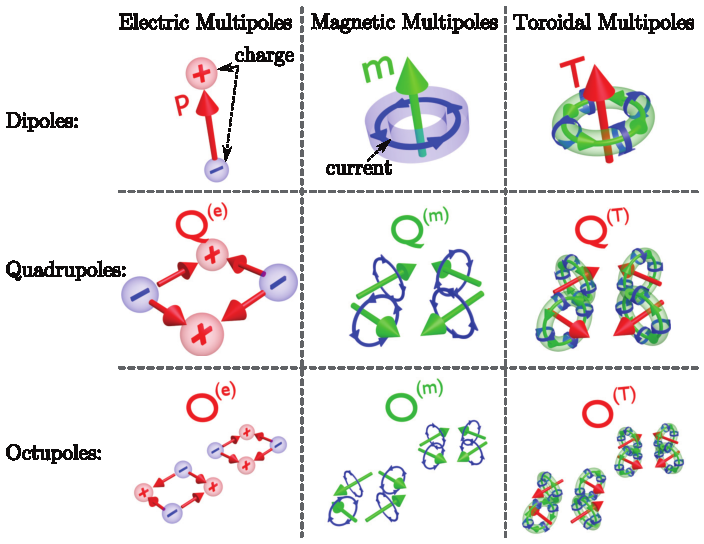
\includegraphics[width=5in]{img/modes2}
	\caption{The three lowest orders of electric, magnetic, and toroidal modes. Adapted from \citein{savinovToroidalDipolarExcitation2014}.}
	\label{fig:modes2}
\end{figure}

In practice these resonances can spectrally overlap and superimpose to form modes observable in the antenna's scattering spectrum (their far-field response). A notable example of this is the anapole mode, for which the toroidal and electric dipoles destructively interfere in the far-field, creating a \emph{dark} mode with low scattering\cite{grinblatEnhancedThirdHarmonic2016}. Mode superpositions can also be utilised to direct the antenna's output through far-field interference.

While this discussion focused on simple antenna shapes, more complex arrangements can be used to achieve various output goals. For example, \citein{krasnokAlldielectricOpticalNanoantennas2012} demonstrates how a set of $\sim$\SI{1}{\micro\meter} diameter silicon spheres laid out in analogy to the Yagi-Uda radio-frequency antenna design can result in output beam-widths as low as \SI{40}{\degree}.

\section{Enhancing nonlinear effects with nanoantennas}
An important advantage of nanoantennas as a nonlinear medium is that their subwavelength size relaxes the phase matching condition\cite{sainNonlinearOpticsAlldielectric2019}, making the design easier and allowing for simplified use of non-birefringent materials. The decreased size results in a disadvantage for nonlinear interactions -- the smaller interaction volume. Beyond the intuitive diminishing of signal when we reduce the amount of material emitting it, there is also the significant dependence of the signal intensity on the interaction length, which can be quadratic in some cases (as seen in Section~\ref{section:nonlinear-optics}). To make up for this we rely on the field enhancing properties of the antennas.

Good field enhancement can be achieved by selecting the correct mode of the antenna. For example, \citein{grinblatEnhancedThirdHarmonic2016} reports that the aforementioned anapole mode in a germanium nanodisk corresponds to a high energy concentration in the antenna; spectral analysis shows that the less scattering is observed, the more energy is confined in the nanoantenna's near-field, highlighting the significance of dark modes. The generated third harmonic intensity when the anapole is excited is predicted and measured to be an order of magnitude greater than for the spectrally close electric dipole resonances, and four orders of magnitude better than from unstructured germanium film. The absolute THG efficiency is given as 0.0001\%.

When choosing a mode to excite in a nanoantenna, it is important to consider where we want the field to be concentrated. The above experiment was concerned with THG, and so field enhancement inside of the antenna was desirable. \citein{cambiassoBridgingGapDielectric2017a} demonstrates a gallium phosphide (GaP) nanodisk for efficient SHG; as GaP is centrosymmetric the field needs to be enhanced at the disk's surface, where second order nonlinear effects can occur. A resonant mode has been found for which the electric field magnitude at the surface is up to 30 times greater than the incident $E_0$. In contrast to the anapole mode, this one corresponds to a peak in scattering. Together with the fact that a GaP substrate with GaP cylinders on it has a larger surface area than the substrate itself, this gives a SHG enhancement by 3 orders of magnitude compared to just the substrate, for an absolute efficiency of 0.0002\%.

The examples above demonstrate that it is important to excite a good mode to fit the desired outcome. Factors other than the antenna shape and the output amplitude can also be considered; for example \citein{koshelevSubwavelengthDielectricResonators2020} demonstrates how adjusting the thickness of an \ch{SiO2} spacer between an AlGaAs nanodisk and a reflective ITO layer, as well as the pump beam shape and polarisation, can help excite a mode referred to as a quasi-BIC (bound state in continuum), leading to a 2-order-of-magnitude increase compared to other implementations of a similar antenna. The choices made in design are also reflected in the output field's shape, as illustrated in Fig.~\ref{fig:directivity}.
\begin{figure}[h]
	\centering
	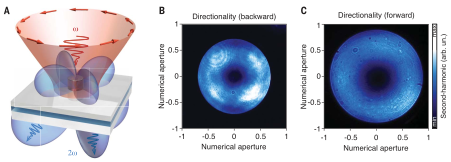
\includegraphics[width=6in]{img/directivity}
	\caption{\textbf{(A)} The pump (red) excites a mode in the nanodisk, which in turn produces second harmonic radiation, shown in blue. \textbf{(B)} and \textbf{(C)} show the far-field intensity of the generated radiation in different directions -- the four lobes from (A) are well pronounced in the backwards-directed generation. Adapted from \citein{koshelevSubwavelengthDielectricResonators2020}.}
	\label{fig:directivity}
\end{figure}

\section{Predicting and optimising the nonlinear signal of an antenna}
Experimental investigation of nonlinear effects is important to capture the full spectrum of their behaviours, as aspects like the material's damage threshold and the way this limits laser pulse duration will not be captured by simulations\cite{koshelevSubwavelengthDielectricResonators2020}. Nevertheless, a thorough computational investigation is an important step in planning and preparing for experimental work, as it allows for exploring arbitrary antenna parameters without manufacturing samples, and for directly looking at field distributions inside the antenna

\subsection{Predicting the field inside of the antenna}
Finite-difference time-domain (FDTD) numerical methods can be used to solve Maxwell's equations when it is hard or impossible to do so analytically. The equations can be rewritten in terms of finite time and distance intervals\cite{kaneyeeNumericalSolutionInitial1966}, and solved numerically to give a description of the fields inside of the structure of interest.

An example of a FDTD solver is the Lumerical 3D Electromagnetic Simulator \cite{lumericalinc.} -- this is the software we are most likely going to use throughout our project.

\subsection{Predicting the third harmonic signal}
Given the polarisation function for a certain material or device, for example \eqref{eq:nonlinear-polarisation}, we can predict its nonlinear signal at a detector for a given pump wave. The method outlined below is known as the nonlinear scattering theory, and the derivation is adapted from the supplementary materials of \citein{obrienPredictingNonlinearProperties2015} and \citein{brunoNegativeRefractionTimevarying2020}.

We start with Lorentz reciprocity, which is the principle stating that exchanging the source and detector of an electric field will not result in a change of the detector's reading. This can be written as an integral over two volumes:
\begin{equation}
	\label{eq:lorentz-rec}
	\int_A\bm{j}_A(\bm{r}_A)\cdot\bm{E}_D(\bm{r}_A)dV_A
	= \int_D\bm{j}_D(\bm{r}_D)\cdot\bm{E}_A(\bm{r}_D)dV_D,
\end{equation}
where $\bm{j}_A$ is the nonlinear contribution to the current density in the antenna induced by the pump, which in turn induces an electric field $\bm{E}_A$. $\bm{j}_D$ is a dummy current dipole placed at the detector, which induces a field $\bm{E}_D$.

By realising that
\begin{equation}
	\label{eq:lorentz-p}
	\bm{j}_A(\bm{r})=\frac{\partial\bm{P}_A(\bm{r})}{\partial t}
	=i\omega\bm{P}_A(\bm{r})
\end{equation}
for a polarisation excited by an electromagnetic wave (the $\bm{P}_A$ here is the nonlinear polarisation of a chosen order, with $\omega$ being the signal frequency), and writing the electric dipole as
\begin{equation}
	\label{eq:lorentz-dipole}
	\bm{j}_D(\bm{r}) = J_0\Delta L\cdot\delta(\bm{r}-\bm{r}_{D0})\hat{\bm{j}}e^{i\omega t},
\end{equation}
where $\hat{\bm{j}}$ is the polarisation axis, $\delta$ the three-dimensional Dirac delta function, $\Delta L$ the dipole's length, and $\bm{r}_{D0}$ its location, we can integrate \eqref{eq:lorentz-rec} to give
\begin{equation}
	\label{eq:lorentz-final}
	\bm{E}_A(\bm{r}_{D0})\cdot\hat{\bm{j}}=
	\frac{i\omega e^{-i\omega t}}{J_0\Delta L}
	\int_A\bm{P}_A(\bm{r}_A)\cdot\bm{E}_D(\bm{r}_A)dV_A,
\end{equation}
which is the electric field signal the detector will see.

Now in order to compute the overlap integral in \eqref{eq:lorentz-final}, we need to know the nonlinear polarisation, and $\bm{E}_D$ at the nanoantenna. These can be obtained using two separate FDTD simulations of the antenna, one for the pump, and one for a dummy field coming from a dipole at the detector (sometimes approximated as a plane wave).

\subsection{Methods of optimising the antenna signal}
Fig.~\ref{fig:steps} schematically shows the many steps that contribute to the final efficiency of nonlinear generation from an antenna. The pump must first couple into the antenna (the efficiency of this depends on the far-field representation of the mode), the mode can be more or less resonant (resulting in various levels of field enhancement), the overlap between the pump and signal modes we're exciting has to be good (see \eqref{eq:lorentz-final}), the signal mode can be further enhanced by resonance, and it should have a strong far-field presence.

\begin{figure}[h]
	\centering
	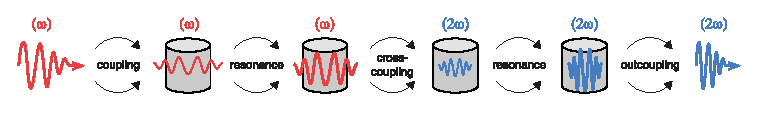
\includegraphics[width=6in]{img/steps}
	\caption{A schematic showing some of the points of possible optimisation for nonlinear generation from an antenna. Adapted from \citein{koshelevSubwavelengthDielectricResonators2020}.}
	\label{fig:steps}
\end{figure}

Each of these steps can be optimised by choosing the appropriate resonances to excite, antenna shape and dimensions, the material it is made of, the operating frequency, and other parameters.

In practice, the parameter space of interest would be first investigated computationally, and then samples would be manufactured and measured to confirm the theory and explore parameters of particular interest. \citein{obrienPredictingNonlinearProperties2015} provides a good example of this; the authors placed a 2D array of antennas on the substrate, with the antenna length and shape varying along the rows and columns respectively. By physically moving the sample so that the pump falls on different antennas they could then sweep a 2-parameter space efficiently.

Another important concept in optimisation is parameter decoupling -- it is for example convenient
to change the nanodisk diameter instead of the pump wavelength\cite{obrienPredictingNonlinearProperties2015, grinblatEnhancedThirdHarmonic2016}. This way we only look at the signal's dependence on the excited mode, not on the spectral properties of the material.

\section{Conclusion}
In this review I covered the basics of nonlinear optics, the fundamental concepts of nanoantennas, and how these two can be combined to utilise effects like harmonic generation on the nanoscale. I have described the results of a number of experiments in the field, each using a slightly different approach to optimising the system's efficiency. I have also shown an overview of a method that can be used to computationally predict the signal output of a nonlinear effect, and gave a brief overview of the parameters of an antenna system that can be focused on to improve its performance.

As our project will be a mix of computational and experimental investigation, we are likely to use the prediction methods shown here, and the insight given by the experiments described in this review. It is evident that there are many possible ways in which nonlinear processes in nanostructures can be enhanced, and we believe our project can be a fruitful exploration of some of the unexplored antenna and substrate parameters and structures.

\bibliographystyle{myIEEEtran}
% argument is your BibTeX string definitions and bibliography database(s)
\bibliography{IEEEabrv,bib.bib}

\end{document}
